% \Section{A fejezet célja}

% Ez a fejezet még nem a saját eredményekkel foglalkozik, hanem bemutatja, mi a problémakör, milyen módszerekkel, milyen eredményeket sikerült elérni eddig másoknak.

% A hivatkozások jelentős része ehhez a fejezethez szokott kötődni.
% (Egy hivatkozás például így néz ki \cite{coombs1987markup}.)
% Itt lehet bemutatni a hasonló alkalmazásokat.

% \Section{Tartalom és felépítés}

% A fejezet tartalma témától függően változhat. Az alábbiakat attól függően különböző arányban tartalmazhatják.
% \begin{itemize}
%   \item Irodalomkutatás. Amennyiben a dolgozat egy módszer kidolgozására, kifejlesztésére irányul, akkor itt lehet részletesen végig nézni (módszertani vagy időrendi bontásban), hogy az eddigiekben milyen eredmények születtek a témakörben.
%   \item Technológia. Mivel jellemzően kutatásról vagy szoftverfejlesztésről van szó, ezért annak a jellemző elemeit, technikai részleteit itt kell bemutatni.
%         Ez tehát egy módszeres bevezetés ahhoz, hogy ha valaki nem jártas a témakörben, akkor tudja, hogy a dolgozat milyen aktuálisan elérhető eredményeket, eszközöket használt fel.
%   \item Piackutatás. Bizonyos témáknál új termék vagy szolgáltatás kifejlesztése a cél.
%         Ekkor érdemes annak alaposan utánanézni, hogy aktuálisan milyen eszközök érhetők el a piacon.
%         Ez szoftverek esetében a hasonló alkalmazások bemutatását, táblázatos formában történő összehasonlítását jelentheti.
%         Szerepelhetnek képek és észrevételek a viszonyításként bemutatott alkalmazásokhoz.
%   \item Követelmény specifikáció. Külön szakaszban érdemes részletesen kitérni az elkészítendő alkalmazással kapcsolatos követelményekre.
%         Ehhez tartozhatnak forgatókönyvek (\textit{scenario}-k).
%         A szemléletesség kedvéért lehet hozzájuk képernyőkép vázlatokat is készíteni, vagy a használati eseteket más módon szemléltetni.
% \end{itemize}

% \Section{Amit csak említés szintjén érdemes szerepeltetni}

% Az olvasóról annyit feltételezhetünk, hogy programozásban valamilyen szinten járatos, és a matematikai alapfogalmakkal sem ebben a dolgozatban kell megismertetni.
% A speciális eszközök, programozási nyelvek, matematikai módszerek és jelölések persze jó, hogy ha említésre kerülnek, de nem kell nagyon belemenni a közismertnek tekinthető dolgokba.

\Chapter{Koncepció}

\Section{Problémakör}

A gamefikáció vagy játékosítás lényege hogy egy adott információt a felhasználó számára játékos formában jelenítsük meg. Ezt az eszközt általában olyan területeken használják amelyek nem annyira játékosak és így próbálják érdekessé, felhasználó baráttá, motiválóvá tenni az adott feladatkört. \vspace{5mm}

A legtöbb rendszer magára a funkcionalitásra fókuszál, hogy elvégezzünk rajta egy meghatározott feladatot a lehető leggyorsabban. Ami munkavégzés szempontjából hatékony, viszont a fogyasztó úgy fogja érezni hogy neki ezt azért kell csinálni mert muszáj, nem azért mert szükségszerűen el akarják látni azt a bizonyos feladatokat.\vspace{5mm}

Ezzel ellentétben az emberközpontú tervezést használó rendszerek használatakor nem érezzük úgy magunkat, hogy az emberek egy kis fogaskerekek egy nagy rendszerben. Az emberközpontú tervezés arra van optimalizálva hogy, motivációs hatása legyen, elkötelezettséget váltson ki belőlünk természetesen az elvégzendő feladat mellett. A valóság az hogy munkával ellentétben játszani nem kötelező, ha nem tetszik egy játék bármelyik pillanatban abba lehet hagyni. Ezért ember központúak a játékok mert a játék készítőinek muszáj lefoglalnia a játékost, ezért van az a sok küldetés, cél és évtizedek alatt kitapasztalt rengeteg játékos elem hogy a játékos ne hagyja abba a játékot. \cite{actionablegamification}.

% Kicsit részletesebben kellene írni ezekről a dolgokról. Lehet mutatni
% a Kahoot-ból és a Duolingo-ból is konkrét példákat, akár képpel együtt,
% hogy mit és milyen formában foglalna magába a tervezett alkalmazás

\Section{Piackutatás}

Napjainkban a két talán legelterjedtem alkalmazást választottam mintául az enyém elkészítéséhez. Az egyik ilyen alkalmazás a Duolingo\cite{duolingo} a másik pedig a Kahoot!\cite{kahoot}, mind a kettőt az oktatást játékosítására hozták létre. \vspace{5mm}

\subsection{Kahoot!}

A Kahoot! tömören egy olyan tanulási platform, amelyen egyszerűen lehet létrehozni, megosztani és kitölteni kvízeket.

De előszöris ahhoz hogy elkészítsük őket először regisztrálni kell, lehet tanár, diák, személyes vagy szakmai fiókot létrehozni. Majd ha ez megvan akkor elkezdhetjük az oldal használatát.

A kvíz készítési része az oldalnak egyszerű, letisztult és intuitív, könnyen lehet kérdéseket hozzáadni és szerkeszteni. Ki tudjuk választani hogy milyen formában szeretnénk szamon kérni a kérdésre a választ a felhasználótól, például 4 válaszlehetőség közül lehet választani egy jót vagy szimplán igaz/hamis állítást feltenni.

\begin{figure}[h]
  \centering
  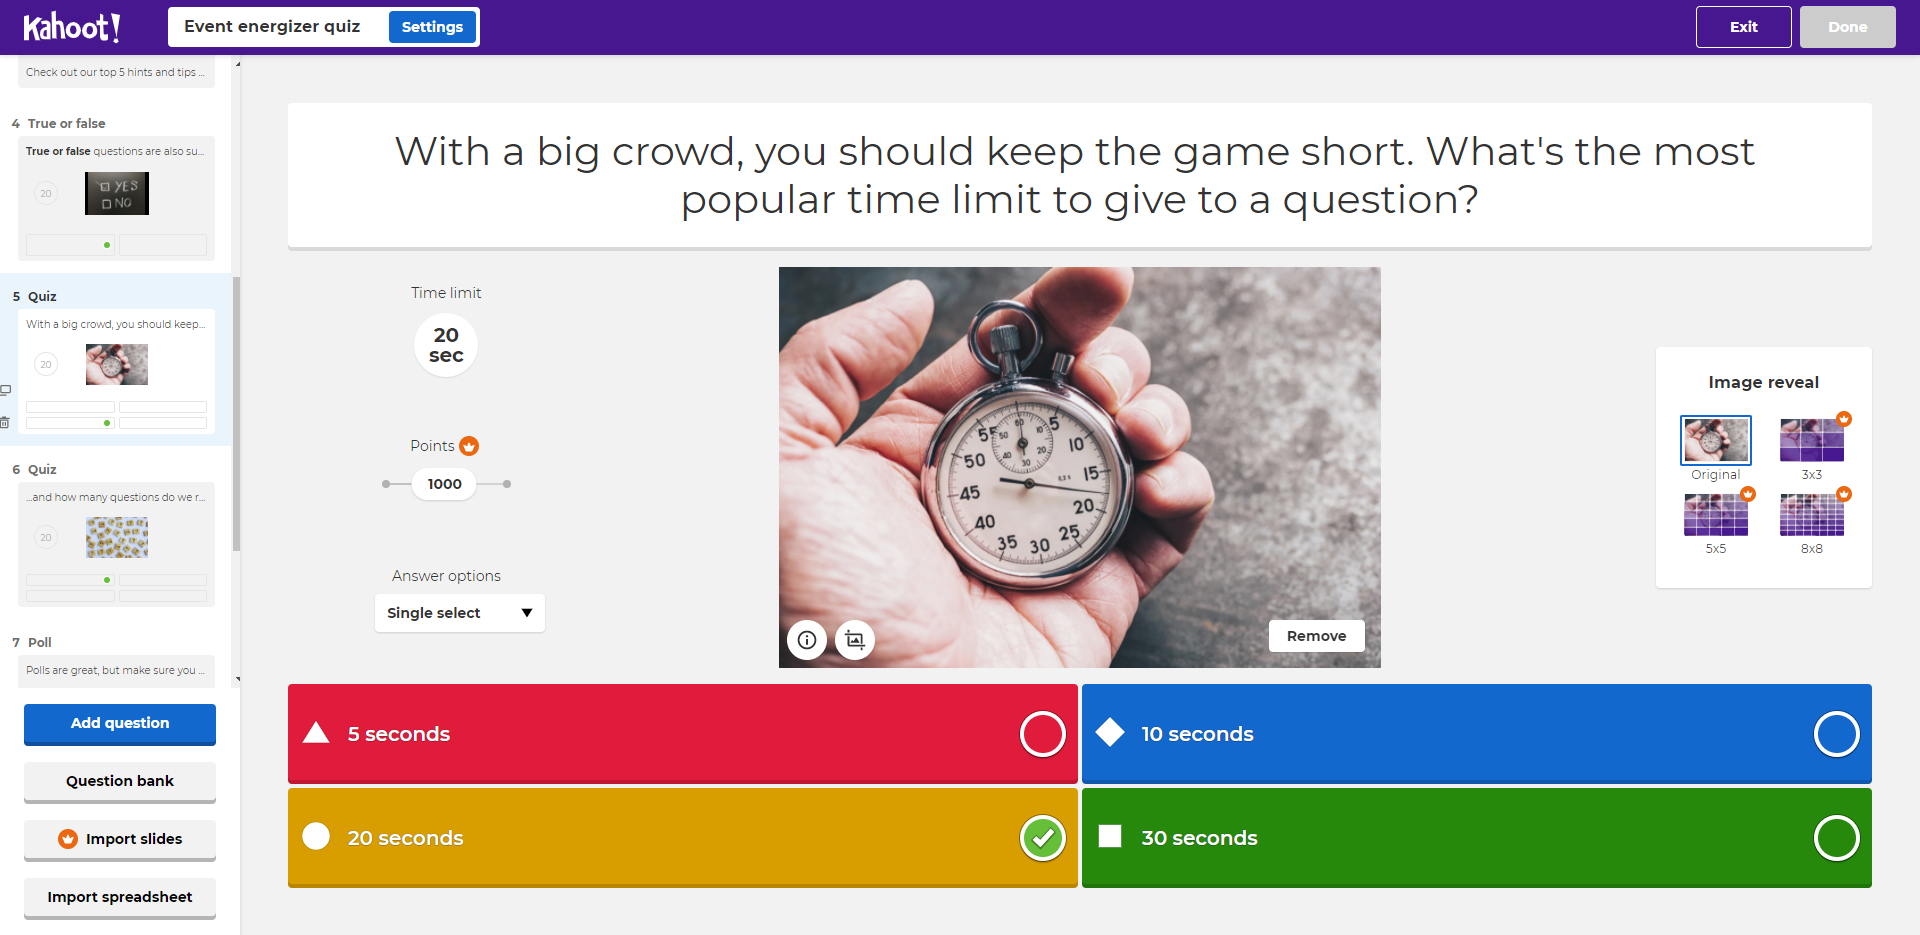
\includegraphics[width=\linewidth]{images/kahoot_test_making.PNG}
  \caption{Teszt készítése Kahoot!-on}
\end{figure}

Majd ha kiválasztottuk megírhatjuk magát a kérdést és a négy válaszlehetőséget és kijelölhetjük melyik a jó válasz. Tudunk beállítani minden kérdéshez idő limitet, hogy hány pontot érjen a kérdésre a helyes válasz, egy vagy több jó válasz legyen és hogy milyen képet szeretnénk a kérdéshez illeszteni.


\begin{figure}[h]
  \centering
  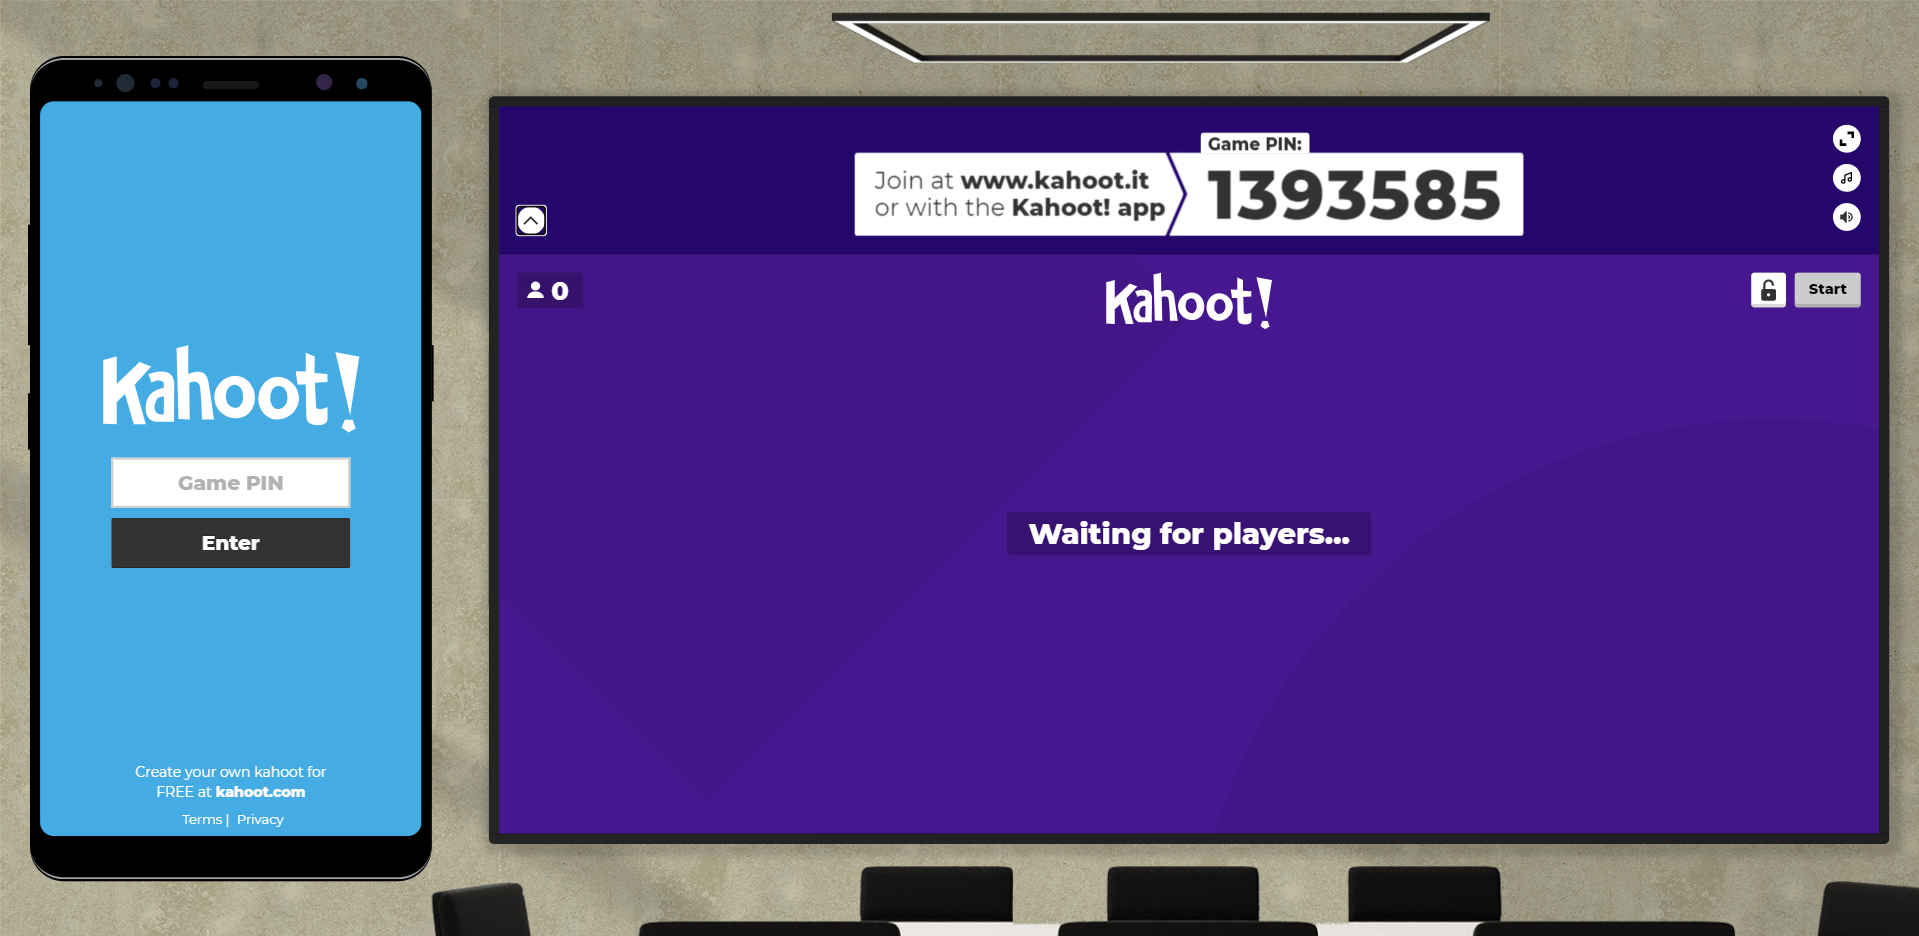
\includegraphics[width=\textwidth]{images/kahoot_play.png}
  \caption{Várakozás játékosokra Kahoot!-on}
\end{figure}
Majd ha kész vagyunk, akkor mások is kitölthetik a tesztünket. Ezt úgy lehet elérni hogy elkészítés után generálódik egy PIN amit a felhasználó beír és már csatlakozhat is. Ha minden felhasználó csatlakozott akkor a teszt készítője elindíthatja a játékot és minden játékos egyszerre látja a kérdéseket és saját eszközén pedig válaszolhat rájuk.


\begin{figure}[h]
  \centering
  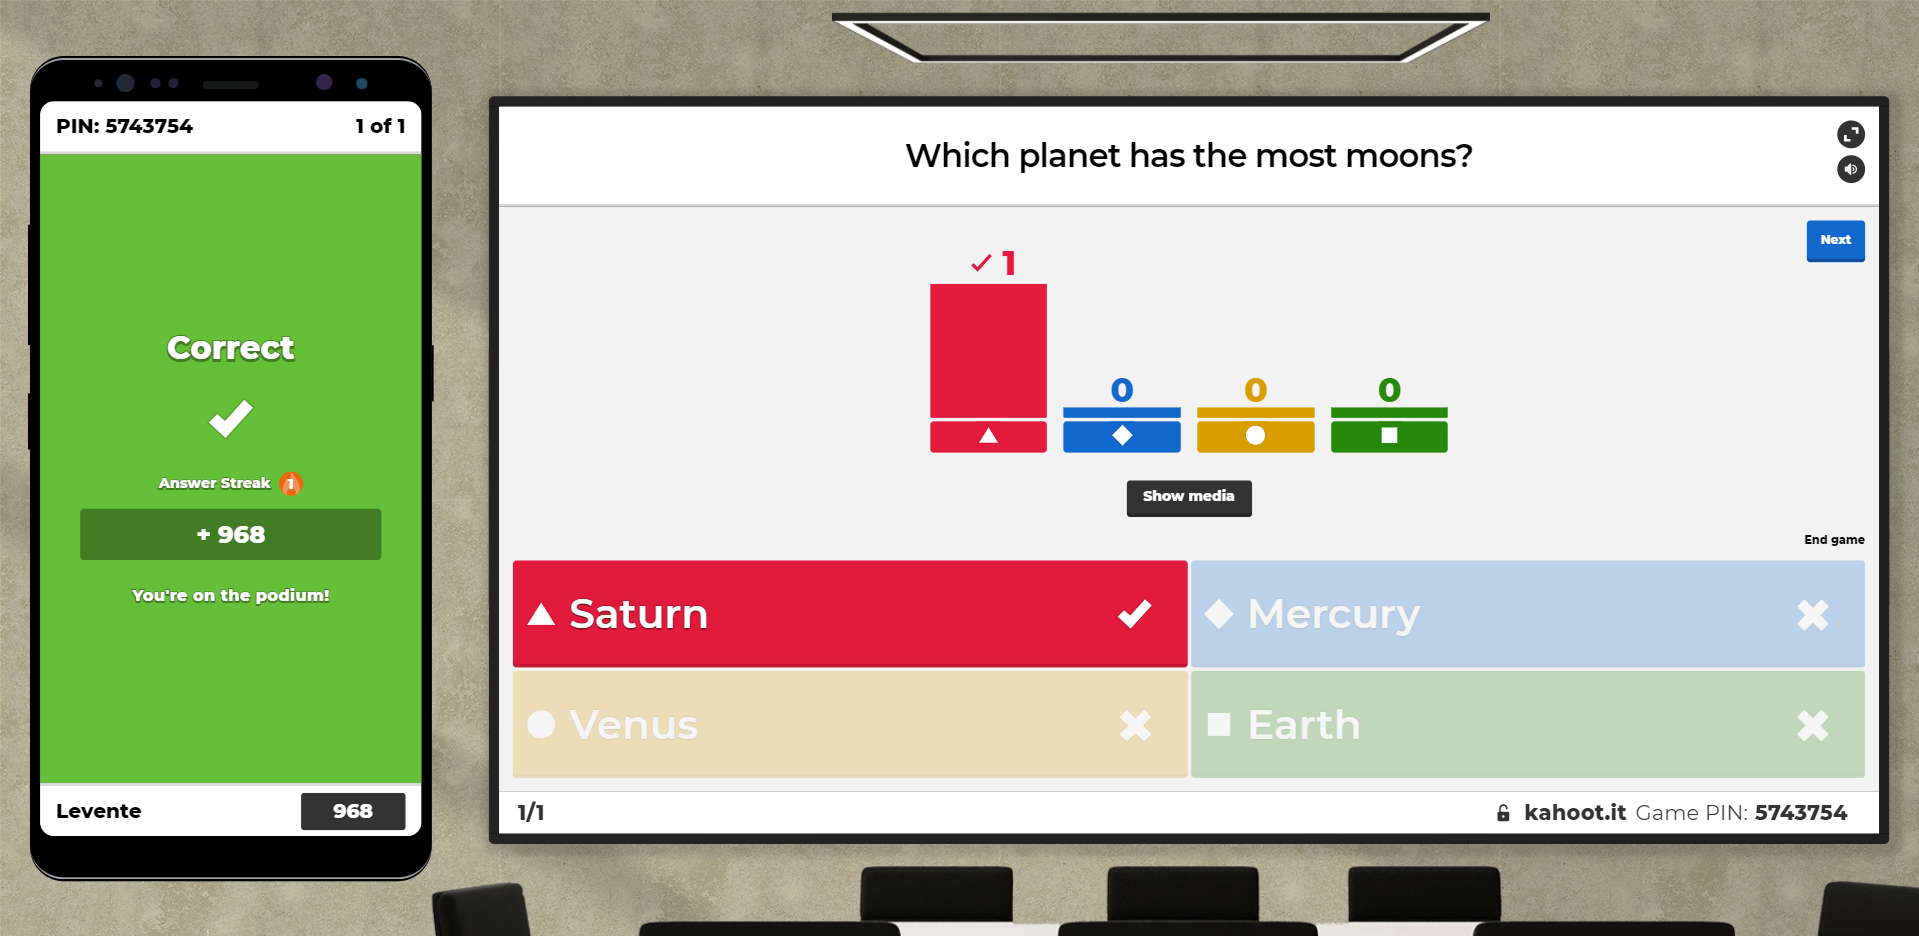
\includegraphics[width=\textwidth]{images/kahoot_play2.png}
  \caption{Válaszadás Kahoot!-on}
\end{figure}
Kérdések után láthatjuk mennyien válaszoltak az adott válaszra és a hogy melyik volt a helyes. Mi magunknak pedig látjuk helyes volt e válaszunk és hogy mennyi pontot szereztünk ezzel a válasszal. Majd a kérdéssorozat után láthatjuk az első három helyezettet és pontjaikat, a játék késztője pedig teljes jelentést nézhet meg a játszott felhasználók teljesítményéről.

\subsection{Duolingo}
A Duolingo a legnépszerűbb nyelvtanulási platform és a legtöbbet letöltött oktatási alkalmazás a világon, több mint 300 millió felhasználóval. Az alkalmazás célja az oktatás ingyenes, szórakoztató és mindenki számára elérhetővé tétele. A Duoling-ót úgy tervezték, hogy úgy érezd egy játékot játszol.\cite{whatIsDuolingo}


\begin{figure}[h]
  \centering
  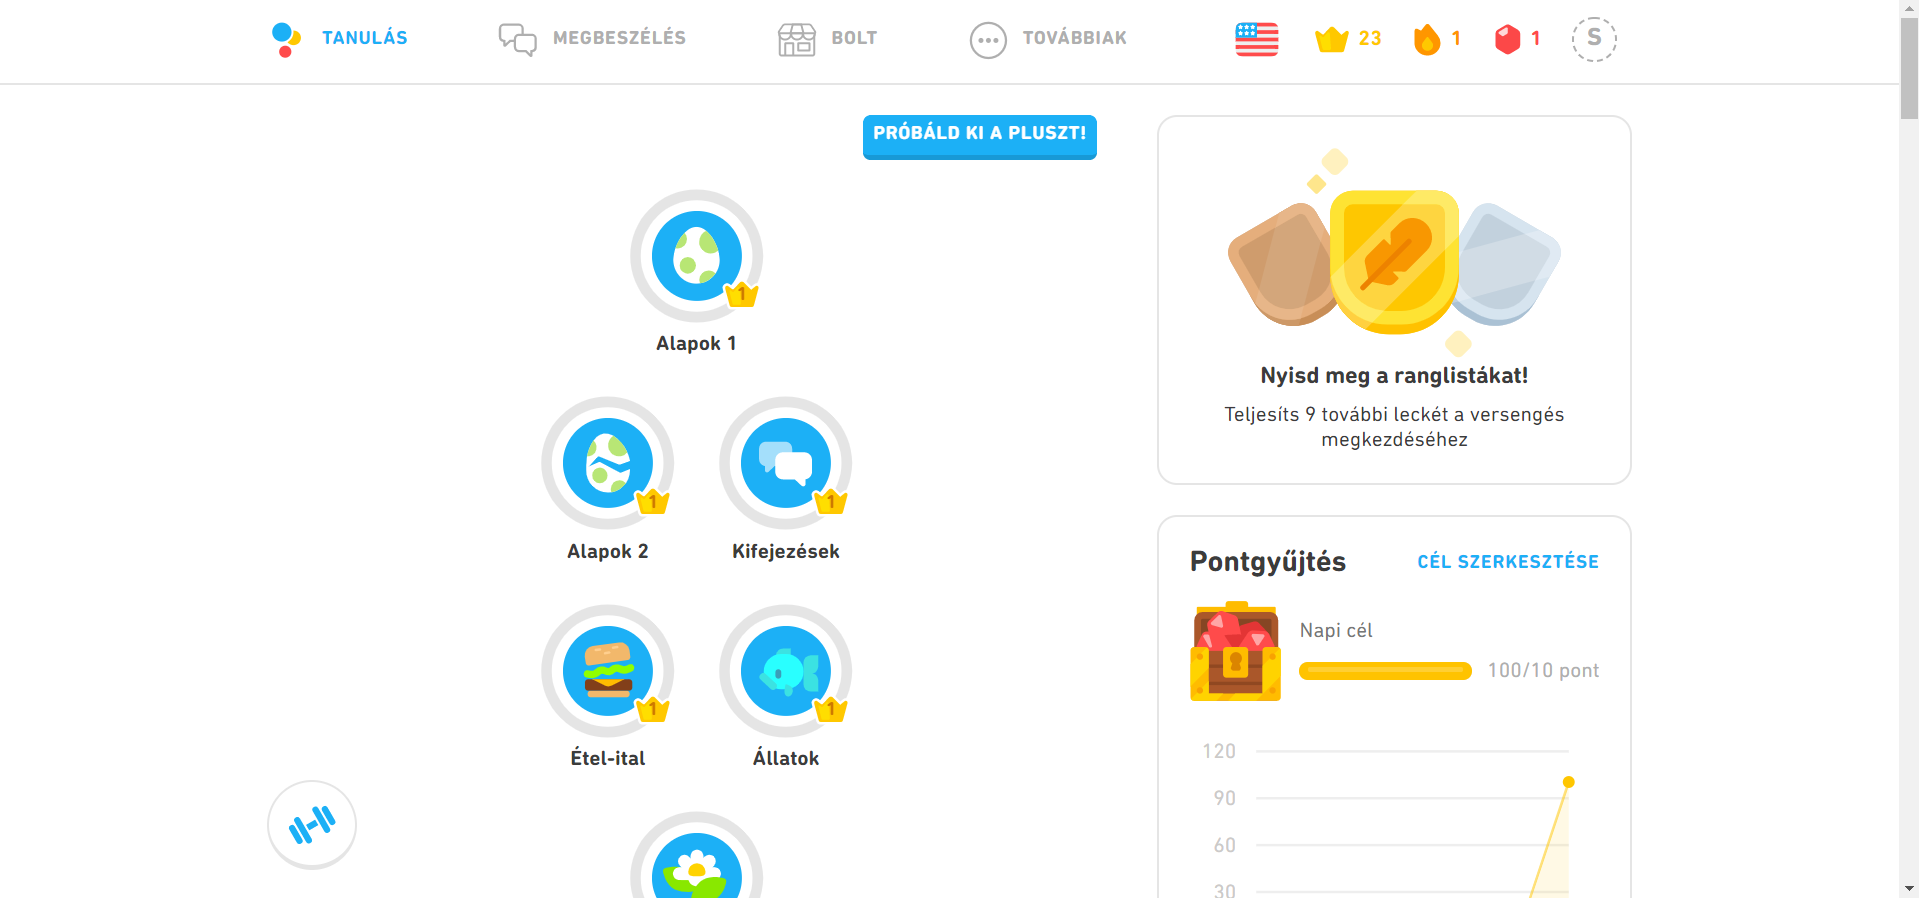
\includegraphics[height=6.8cm]{images/Duolingo_main_page.png}
  \caption{Válaszadás Kahoot!-on}
\end{figure}

A felületem is már látszik hogy játékos és hogy játékokból vett elemekkel van megtűzdelve az egész oldal. Például:
\begin{itemize}
  \item {Pontgyűjtés}
        \begin{addmargin}[\parindent]{0pt}
          Tanulás során pontokat lehet szerezni, amelyeket tapasztalati pontoknak neveznek. Ezeket leckék elvégzésével, ismeretanyag gyakorlásával vagy például szintugró-teszt elvégzésével lehet.
        \end{addmargin}
  \item Napi cél
        \begin{addmargin}[\parindent]{0pt}
          A napi cél a motiváció megőrzésére szolgál, beállíthatjuk hogy naponta hány pontot szeretnénk szerezni tanulással. Napi jutalmat lehet megkapni, amikor teljesíted a kitűzött célt.
        \end{addmargin}
  \item Koronák
        \begin{addmargin}[\parindent]{0pt}
          Minden ismeretanyaghoz tartozik egy koronaszint. Ha szintet lépsz egy ismeretből, akkor Koronát szerzel, és a feladatok egyre nehezebbek lesznek. Dönthetsz úgy, hogy mélyebben beleásod magad egy ismeretanyagba, és megpróbálsz magasabb szintre jutni, vagy egy új ismeretanyagot is megnyithatsz, hogy új tartalmakat tanulhass. \cite{koronaszintekDuolingo}.
        \end{addmargin}
  \item Széria
        \begin{addmargin}[\parindent]{0pt}
          A széria a napok számát jelzi amelyek során minden egymást követő napon el lett végezve egy lecke. Miután befejeztük a leckét az alkalmazásban vagy a weboldalon, a széria 1 nappal növekszik. Egy kis tűz vagy láng ikon jelképezi a szériát. Amíg el nem éred a napi célodat, szürkén jelenik meg. A napi lecke elvégzése után színessé válik. \cite{szeriaDuolingo}
        \end{addmargin}
  \item Barátok
        \begin{addmargin}[\parindent]{0pt}
          Lehetnek az alkalmazáson belül barátaid akiknek láthatod az elért eredményeit és követhetitek egymást ezáltal látva egymás fejlődését.
        \end{addmargin}
  \item Ranglista
        \begin{addmargin}[\parindent]{0pt}
          A ranglisták egy olyan, amely segítségével versenyezhetsz a többi nyelvtanulóval egy ligán belül. Pontokat lehet szerezni és ezáltal feljutni a ranglista csúcsára. Ezután a ranglistán szereplő tíz legjobban teljesítő felhasználó a következő héten magasabb szintre lép. Az utolsó tíz felhasználó pedig az előző szintre kerül vissza.
        \end{addmargin}
\end{itemize}

\section{Eddigi eredmények felhasználása}
A saját alkalmazásomba bele szeretném vinni előzőleg bemutatott mindkét alkalmazásból a következőket:

% Ez a rész fejlesztés során még változhat egyenlőre csak egy koncepció 
\begin{itemize}
  \item {Tesztkészítés}
        \begin{addmargin}[\parindent]{0pt}
          Kahoot!-hoz hasonló teszt készítési felületet szeretnék létrehozni ahol az elkészített teszthez egy egyedi azonosító generálódik ami alapján el lehet küldeni diákoknak és ezután kitölthetik.
        \end{addmargin}
  \item {Pontgyűjtés}
        \begin{addmargin}[\parindent]{0pt}
          Minden regisztrált felhasználó rendelkezik majd egy szinttel és egy bizonyos pontszámmal, amelyet a tesztek kitöltésével szerezhetnek.
        \end{addmargin}
  \item {Ranglista}
        \begin{addmargin}[\parindent]{0pt}
          Ranglista a teszt teljes kitöltést követően alakul ki a megtöbbet szerzett pontok alapján.
        \end{addmargin}
  \item {Felhasználói szerepkörök kezelése}
        \begin{addmargin}[\parindent]{0pt}
          Különböző szerepkörök lennének amik azzal bírnának hogy egy tanár jogosultságú felhasználó hozhat létre tesztet és hozzá rendelheti diákokhoz. A diák pedig csak kitölthetné azt.
        \end{addmargin}
\end{itemize}